\documentclass[a4paper, 12pt]{article}
\usepackage[a4paper, rmargin=3cm, lmargin=3cm, top=2.5cm, bottom=2.5cm]{geometry}
\usepackage{mathtools}
\usepackage{bookmark}
\usepackage{subcaption}
\usepackage{amsthm,amsmath,amssymb}
\usepackage{enumitem}
\usepackage[ruled, noline]{algorithm2e}
\usepackage{fontspec}

\usepackage{setspace}
\setstretch{1.5}
\setlength{\parindent}{1.25cm}
\setlength{\parskip}{6px}

\usepackage{unicode-math}
\setmathfont{Stix Two Math}
\setmathfont{TeX Gyre Pagella Math}[
   range=bb,
   Scale=MatchUppercase,
   version=pagella
]

\usepackage{polyglossia}
\setdefaultlanguage{portuguese} % might be portuguese, though referencing may present incompatibilities
\setotherlanguages{english} % secondary language for abstract and stuff
\usepackage{times} % not recommended, but it is the standard package for Times included in LuaTeX and ready to go for Overleaf, see alternative option below (which require local installation of LaTeX)

% in case you have a local installation for the font Times, this is preferrable, especially if you have Small Caps support
%\setmainfont{times}[
%  % In my case, needs to point for MS Office location since regular MacOS Times doesn't support small caps
%  Path           = /Applications/Microsoft Word.app/Contents/Resources/DFonts/,
%  Extension      = .ttf ,
%  BoldFont       = *bd ,
%  ItalicFont     = *i ,
%  BoldItalicFont = *bi,
%  Ligatures      = Rare, %for some unknown reason, Times put Common ligatures under Rare
%]

% or simply, in case you have the legal font Times LT Std installed in your local machine
%\setmainfont{Times LT Std}[Ligatures = Common] % name might differ

% useful command defition for writting mathematics: QED, norm, set cardinality and equals by definition
\renewcommand{\qedsymbol}{$\blacksquare$}
\newcommand{\norm}[1]{\left\lVert#1\right\rVert}
\newcommand{\card}[1]{\lvert#1\rvert}
\newcommand*{\defeq}{\mathrel{\vcenter{\baselineskip0.5ex \lineskiplimit0pt
                     \hbox{\scriptsize.}\hbox{\scriptsize.}}}%
                     =}

% useful command definition for SCB bracket citation
\newcommand{\citeb}[1]{\bibleftbracket\cite{#1}\bibrightbracket}

% math numbering scheme, speak with your supervisor in case you want to change it
\newtheorem{theorem}{Theorem}[section]
\newtheorem*{definition}{Definition}
\newtheorem{corollary}{Corollary}[theorem]
\newtheorem{lemma}[theorem]{Lemma}


% reference style (Sociedade Brasileira de Computação is compliant with Chicago author-date)
% as per https://presencial.unifcv.edu.br/arquivos/orientacao_para_artigos_area_informatica.pdf
\usepackage[authordate, strict, backend=biber, autolang=other]{biblatex-chicago}
\addbibresource{references.bib}
\DeclareDelimFormat{nameyeardelim}{\addcomma\space}
\setlength\bibitemsep{6.0pt}

% flush all sections right
\usepackage{sectsty}
\sectionfont{\raggedleft}

% used only for text samples, can be safely removed in the final document
\usepackage{lipsum} 
\usepackage{metalogo}

% used for image rendering
\usepackage{graphicx}
\graphicspath{ {../images/} }

\begin{document}
% Page numbering for early pages and document presentation
\pagenumbering{roman}
\setcounter{page}{1}

\thispagestyle{empty}
    \begin{center}
        
\includegraphics[scale=0.18]{../images/unirio.png}\\
        \fontsize{13}{15}
        \textsc{
            Universidade Federal do Estado do Rio de Janeiro\\
            Centro de Ciências Exatas e Tecnológicas\\
            Escola de Informática Aplicada\\
        }
        \vspace{2.8cm}
        Retrieval Augmented Generation Aplicada à Bibliotecas\\
        \vspace{2.8cm}
        Breno Costa da Silva Filgueiras
        \vspace*{\fill}\\
        
        \textsc{Rio de Janeiro, RJ -- Brasil\\ Dezembro, 2024}
    \end{center}
    \clearpage

    \begin{center}
        Retrieval Augmented Generation Aplicada à Bibliotecas
        \vskip 0.5cm
        Breno Costa da Silva Filgueiras
        \vskip 2.0cm
    \end{center}
    \begin{flushright}
        \parbox{8.0cm}{
        Projeto de graduação apresentado à Escola de Informática Aplicada
        da Universidade Federal do Estado do Rio de Janeiro (UNIRIO) como
        cumprimento de requerimento parcial para obtenção título de Bacharel em
        Sistemas de Informação.}
        \vskip 1.5cm
        Approved by:
        \vskip 1.5cm
        \rule{10.0cm}{.1mm}

        Supervisor, D.Sc. -- UNIRIO
        \vskip 1.0cm

        \rule{10.0cm}{.1mm}

        Supervisor 2, D.Sc. -- UNIRIO
        \vskip 1.0cm

        \rule{10.0cm}{.1mm}

        Supervisor 3, D.Sc. -- XXXX
        \vskip 1.0cm
    \end{flushright}
    \vspace{\stretch{1}}
    \begin{center}
        \textsc{Rio de Janeiro, RJ -- Brasil} \\ \textsc{Dezembro, 2024}
    \end{center}
    % Fim da folha de rosto

    \clearpage
    \begin{flushright}
        Agradecimentos
    \end{flushright}
    \lipsum[1-2]
    \clearpage

    \begin{abstract}
        Em uma parceria entre Seagate e a International Data Corporation (IDC) foi realizado o estudo “The Digitization of the World From Edge to Core”, nele a IDC fala sobre diversos aspectos referentes aos dados presentes no mundo digital e um dos tópicos abordados no estudo é “Mankind is on a quest to digitize the world” e neste mesmo tópico eles explicam que os dados que geramos no dia a dia está em constante crescimento, ou seja, estamos gradualmente produzindo mais dados.

        Com um volume cada vez maior de dados, uma busca por informação otimizada é essencial, dado que são necessárias ferramentas que nos garantam confiança e precisão da informação adquirida. Com isso em mente, este trabalho visa o desenvolvimento de um sistema capaz de ler, processar e armazenar documentos diversos de determinada biblioteca (conjunto de documentos) para que possamos utilizar um Large Language Model (LLM) para responder perguntas que os usuários possam ter acerca dos documentos.
        
        A ideia é conseguir processar documentos de diferentes épocas, temas, formatos e conseguir responder o maior número possível de perguntas dos usuários com a melhor confiança possível.

        \begin{flushleft}
            \textbf{Palavras-chave:} retrieval, augmented, generation, inteligência, artificial.
        \end{flushleft}
    \end{abstract}
    \clearpage

    \begin{english}
        \begin{abstract}
            In a partnership between Seagate and the International Data Corporation (IDC), the study “The Digitization of the World From Edge to Core” was conducted. In it, IDC discusses various aspects related to data present in the digital world and one of the topics covered in the study is “Mankind is on a quest to digitize the world”. In this same topic, they explain that the data we generate on a daily basis is constantly growing, that is, we are gradually producing more data.

            With an ever-increasing volume of data, an optimized search for information is essential, given that tools are needed that guarantee reliability and accuracy of the information acquired. With this in mind, this work aims to develop a system capable of reading, processing and storing various documents from a given library (set of documents) so that we can use a Large Language Model (LLM) to answer questions that users may have about the documents.

            The idea is to be able to process documents from different periods, themes and formats and to be able to answer as many user questions as possible with the greatest possible confidence.

            \begin{flushleft}
                \textbf{Keywords:} retrieval, augmented, generation, artifical, inteligence.
            \end{flushleft}
        \end{abstract}
    \end{english}
    \clearpage

    \tableofcontents
    \clearpage

    \listoffigures
    \clearpage

    \listoftables
    \clearpage

    \listofalgorithms
    \clearpage

    \pagenumbering{arabic}
    \setcounter{page}{1}

    \section{Introdução}

    \subsection{Motivação}
    Recentemente precisei implementar uma solução de onboarding para funcionários de uma determinada empresa. Por ser uma empresa grande, diversas regras e normas estavam distribuidas em inúmeros documentos (documentos de formatos distintos e sem uma padronização específica), o que gerava uma dor para funcionários recém contratados, que nem sempre sabiam qual documento consultar.

    Para implementar esta solução, foi escolhida uma abordagem que utilizasse o conceito de Retrieval Augmented Generation (RAG) para trazer aos funcionários a informação buscada no menor tempo possível e com confiança de que a informação é válida. Ao longo da implementação da solução, lembrei de todas as vezes que precisei ler um artigo, livro ou até slides só por conta de um determinado tópico ou assunto e o tempo que gastei procurando uma informação que nem sempre seria útil, seja por falta de referência ou a própria informação.

    Com isso em mente, busquei implementar um projeto que seria capaz de processar uma biblioteca de documentos e implementar o conceito de RAG para que um usuário seja capaz de fazer perguntas em uma interface de chat simples e com base nos dados processados da biblioteca de documentos, um Large Language Model (LLM) irá retornar uma resposta humanizada contendo uma resposta e a referência, de qual documento veio a resposta, ao usuário.

    O tema de busca por informação é importante, pois na internet ainda encontramos diversos dados sem referência ou representados de maneiras distintas (como em um gráfico e em um texto descritivo, ambos com a mesma informação), alguns dados também podem estar alocados em aplicações pouco intuitivas o que acaba aumentando o tempo de busca por informação, seja um site difícil de navegar ou um portal com o mecanismo de busca ruim. Todo esse tempo investido na busca por uma informação, nem sempre é vantajoso para estudantes e pesquisadores, o que pode dificultar pesquisas e trabalhos a longo prazo.

    \subsection{Objetivos}
    O principal objetivo deste trabalho é provar que é possível implementar uma solução RAG para bibliotecas de documentos específicos, neste caso os Trabalhos de Conclusão de Curso (TCCs), disponíveis na biblioteca de publicações do curso de Bacharelado em Sistemas de Informação (BSI) da Universidade Federal do Estado do Rio de Janeiro (UNIRIO) [\textcite{tccs_unirio}].

    Mais especificamente, estarei usando como biblioteca todos os TCCs de 2023 disponíveis na biblioteca do curso. Embora sejam do mesmo curso e ano, nem todos os trabalhos possuem a mesma estrutura, os alunos são livres para escrever seus trabalhos de diversas formas e não há como garantir uma padronização comum à eles, tornando o processamento dos documentos mais complexo. No entanto, todos os documentos disponíveis na bibliotecas são do tipo Portable Document Format (PDF) com extensão .pdf, isso vai contribuir durante a etapa de implementação dos extratores mais a frente no projeto.
    
    \subsection{Metodologia}
    Neste projeto irei utilizar uma abordagem de Design Science Research (DSR) para que ao final do projeto o artefato modelado esteja implementado e funcionando como planejado.

    O DSR tem suas raízes na engenharia e nas ciências do artificial [\textcite{simon_1996}]. É uma metodologia fundamental para a resolução de problemas, buscando aprimorar o conhecimento humano com a criação de artefatos inovadores e a geração de conhecimento de design por meio de soluções para problemas do mundo real [\textcite{design_science}].
    
    Deste modo, ao utilizar o DSR, ao final do projeto haverá um artefato que foi produzido com base na aplicação de tudo estudado e discutido nas próximas seções deste trabalho.
    
    \clearpage

    \section{Fundamentação}

    \subsection{Conceitos Fundamentais}

    No livro RAG-Driven Generative AI, do Denis Rothman, ele diz que "Mesmo o modelo mais avançado de Inteligêcia Artificial (IA) generativa é limitado a responder sobre dados nos quais ela foi treinada." \textcite{rothman} o que nos chama a atenção a um probelma em especial, como fazer para que uma IA saiba responder perguntas referentes a um conjunto específico de dados?

    De fato, uma IA não tem como saber o que ela não sabe, não existe conhecimento além dos dados nos quais ela foi treinada. Perguntas fora do contexto do treinamento de uma IA geralmente levam a halucinações, viés e respostas sem sentido. Para isso, foi implementado um framework, ou estrutura, que combina abordagens baseadas em recuperação com modelos generativos, esta estrutura é a Retrieval Augmented Generation (RAG).

    A RAG recupera dados relevantes de fontes externas em tempo real e usa esses dados para gerar respostas contextualmente relevantes. Uma de suas principais vantagens é a adaptabiolidade, tendo em vista que a estrutura pode ser aplicada independente do tipo de dado abordado na solução, seja texto, imagens, áudios ou documentos diversos.

    \subsection{O que é RAG?}
    
    Quando um modelo de IA generativa não sabe responder determinada pergunta com precisão, diz-se que ele está alucinando ou apresentando viés, mas, na prática, está apenas gerando respostas sem sentido. Isso ocorre porque o modelo não foi treinado com as informações solicitadas ou por conta de limitações em sua configuração, resultando em sequências prováveis, mas não precisas necessariamente.

    A RAG começa onde a IA generativa termina, fornecendo informações que um modelo de LLM não possui para responder com precisão. A RAG otimiza tarefas de recuperação de informações e adiciona os dados recuperados durante a entrada (seja consulta do usuário ou um prompt automatizado), gerando uma saída melhorada e mais amigável ao usuário. O funcionamento geral do RAG pode ser resumido na figura a seguir:

    \begin{figure}[h]
        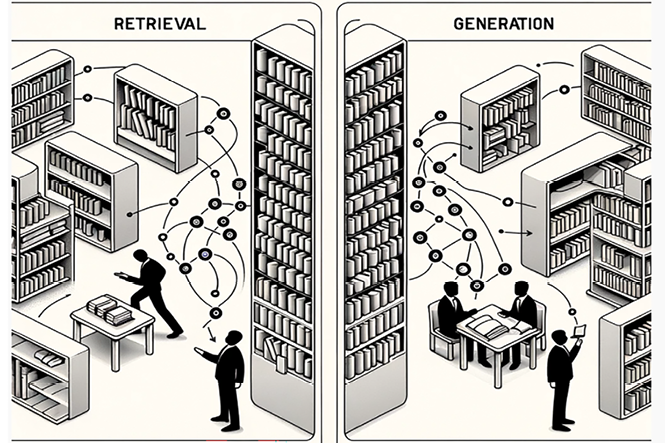
\includegraphics{retrieval-generation.png}
        \centering
        \caption{Funcionamento geral de uma estrutura RAG}
        \centering
    \end{figure}

    Imagine um estudante em uma biblioteca, com a tarefa de escrever uma dissertação sobre RAG. Assim como o ChatGPT ou outros copilotos de IA, o estudante sabe ler e escrever. Como qualquer LLM, ele é treinado para compreender informações avançadas, resumir e criar conteúdo. No entanto, como qualquer IA avançada, seja do Hugging Face, Vertex AI ou OpenAI, há muitas informações que este estudante ainda desconhece.

    Na fase de recuperação, ele busca por livros sobre o tema necessário (lado esquerdo da figura 1) na biblioteca. Em seguida, ele retorna ao seu lugar, realiza a tarefa de recuperação sozinho ou com a ajuda de um colega, extraindo as informações relevantes dos livros adquiridos. Na fase de geração (lado direito da figura 1), o estudante começa a escrever sua dissertação. Assim, funciona como um agente humano guiado por RAG, de maneira semelhante a um framework de IA generativa baseado em RAG.

    Enquanto escreve o seu ensaio sobre RAG, o estudante encontra tópicos difíceis com os quais não tem tempo para consultar todas as informações disponíveis. Como um agente humano generativo, ele fica travado, assim como um modelo de IA generativa. Ele até pode tentar escrever algo, mas, como a IA, não saberá se o conteúdo está correto até que alguém corrija a dissertação e lhe avalie de alguma maneira.

    Neste ponto, ele já atingiu seu limite e decide recorrer a um copiloto de IA generativa com RAG para obter respostas corretas. No entanto, existe uma variedade tão grande de modelos LLM e configurações RAG disponíveis que o estudante acaba ficando confuso. Antes de prosseguir, é necessário entender os recursos disponíveis e como o RAG está organizado.

    \subsection{Ecossistema RAG}

    A IA generativa baseada em RAG é um framework que pode ser implementado com diversas configurações, funcionando dentro de um ecossistema amplo (Figura 2). Independentemente da quantidade de frameworks de recuperação e geração disponíveis, tudo se resume a quatro domínios principais e suas respectivas questões:
    
    \begin{itemize}
        \item Dados: De onde vêm os dados? São confiáveis e suficientes? Há questões de direitos autorais, privacidade ou segurança?
        \item Armazenamento: Como os dados serão armazenados antes ou depois do processamento? Qual será o volume armazenado?
        \item Recuperação: Como os dados corretos serão recuperados para complementar o input do usuário? Qual tipo de framework RAG será mais adequado ao projeto?
        \item Geração: Qual modelo de IA generativa melhor se adapta ao framework RAG escolhido?
    \end{itemize} 

    Esses domínios dependem do tipo de framework RAG utilizado. Antes de escolher, é essencial avaliar a proporção de conhecimento paramétrico e não paramétrico no ecossistema implementado. A Figura 1.3 ilustra os principais componentes do framework RAG, independentemente do tipo implementado.

    \begin{figure}[h]
        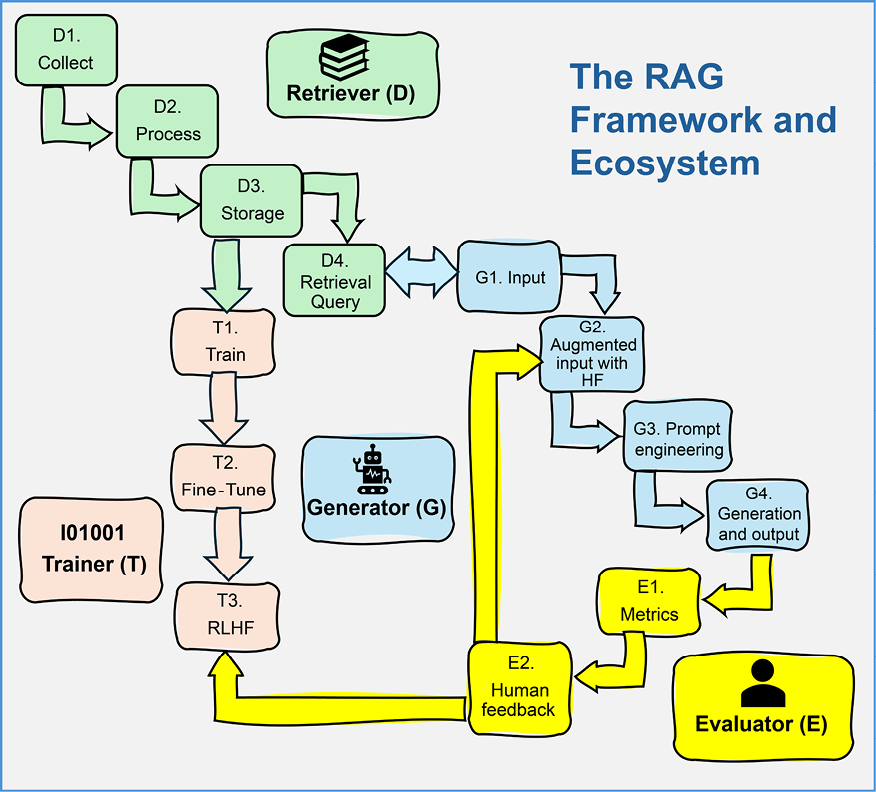
\includegraphics{rag-framework-ecosystem.png}
        \centering
        \caption{Arquitetura da estrutura RAG}
        \centering
    \end{figure}

    \begin{itemize}
        \item Retriever (D): Responsável pela coleta, processamento, armazenamento e recuperação de dados.
        \item Generator (G): Cuida da complementação do input, engenharia de prompts e geração de respostas.
        \item Evaluator (E): Avalia o desempenho usando métricas matemáticas, feedback humano e outras formas de validação.
        \item Trainer (T): Gerencia o modelo pré-treinado inicial e sua posterior fine-tuning.
    \end{itemize}

    Esses quatro componentes dependem de seus respectivos ecossistemas, formando o pipeline de IA generativa baseada em RAG. Nas seções a seguir, usaremos as siglas D, G, E e T para representar respectivamente Retriever, Generator, Evaluator e Trainer. Começando pelo Retriever (D).

    \subsubsection{Retriever (D)}

    O componente retriever de um ecossistema RAG coleta, processa, armazena e recupera dados. O ponto de partida de um ecossistema RAG é, portanto, um processo de ingestão de dados, cujo primeiro passo é a coleta de dados.

    \begin{enumerate}
        \item Coleta de Dados (D1):\\
        Atualmente dados são extremamente diversos, podendo ser textos, arquivos de mídia (como músicas ou vídeos em mp4) ou arquivos estruturados e não estruturados (PDFs, JSONs e páginas web). Além disso, grande parte desses dados é não estruturada e pode ser encontrada de maneiras imprevisíveis e complexas. Felizmente, várias plataformas, como Pinecone, OpenAI, Chroma e Activeloop, oferecem ferramentas prontas para processar e armazenar essa vasta quantidade de dados.
        \item Processamento de Dados (D2):\\
        Na fase de coleta de dados (D1) no processamento de dados multimodais, diferentes tipos de dados, como texto, imagens e vídeos, podem ser extraídos de websites utilizando técnicas de web scraping ou outras fontes de informação. Esses objetos de dados são então transformados para criar representações uniformes. Alguns exemplos dessas transformações incluem: chunking, embedding e indexação. Essas técnicas serão discutidas mais adiante.
        \item Armazenamento de Dados (D3):\\
        Neste estágio do pipeline, já coletamos e começamos a processar uma grande quantidade de dados diversos. Mas para fazermos com que esses dados para sejam úteis, vamos fazer uso de vetor stores (armazenamento de vetores), como Elastic Search. Ele não apenas armazena os dados, mas os convertem em entidades matemáticas, representadas como vetores, permitindo realizar cálculos poderosos. Esses sistemas também utilizam técnicas de indexação e outras abordagens para garantir acesso rápido e eficiente aos dados. Em vez de manter os dados em arquivos estáticos, transformamos tudo em um sistema dinâmico e pesquisável, pronto para alimentar chatbots, motores de busca e outras aplicações.
        \item Consulta de Recuperação (D4):\\
        O processo de recuperação é acionado pelo input do usuário ou input automatizado (G1). Para recuperar dados rapidamente, carregamos os dados nos vetor stores e datasets após transformá-los para um formato adequado. Em seguida, utilizamos uma combinação de pesquisas por palavras-chave, embeddings inteligentes e indexação para recuperar os dados de forma eficiente. 
        A similaridade cosseno, por exemplo, encontra itens que estão intimamente relacionados, garantindo que os resultados da busca não sejam apenas rápidos, mas também altamente relevantes.
        Após a recuperação dos dados, o próximo passo é aumentar o input, ou seja, adicionar as informações recuperadas para enriquecer a resposta gerada.
    \end{enumerate}

    \subsubsection{Generator (G)}

    No ecossistema RAG, as linhas entre a entrada e a recuperação não são tão nítidas, como mostrado na figura 2, que representa o framework e ecossistema RAG. O input do usuário (G1), seja automatizado ou humano, interage com a consulta de recuperação (D4) para complementar o input antes de enviá-lo ao modelo generativo. O fluxo gerativo começa com o input, que é aprimorado com dados recuperados antes de ser processado pelo modelo de IA generativa.

    \begin{enumerate}
        \item Entrada (G1):\\
        O input pode ser uma série de tarefas automatizadas (como o processamento de e-mails, por exemplo) ou prompts humanos por meio de uma Interface de Usuário (UI). Essa flexibilidade permite integrar a IA de forma fluida em diversos ambientes profissionais, aprimorando a produtividade em diferentes setores.
        \item Entrada Aumentada com Feedback Humano (G2):\\
        O feedback humano (HF, de Human Feedback) pode ser adicionado ao input, conforme descrito na seção Feedback Humano (E2), sob o componente Evaluator (E). O feedback humano torna o ecossistema RAG consideravelmente mais adaptável, permitindo total controle sobre a recuperação de dados e os inputs para a IA generativa. Na seção Building Hybrid Adaptive RAG in Python deste capítulo, construiremos o input aumentado com feedback humano, melhorando a precisão e a relevância das respostas geradas.
        \item Engenharia de Prompts (G3):\\
        Tanto o retriever (D) quanto o generator (G) dependem fortemente da engenharia de prompts para preparar a mensagem padrão e aumentada que o modelo de IA generativa deverá processar. A engenharia de prompts combina a saída do retriever com o input do usuário, garantindo que o modelo receba uma entrada bem estruturada e relevante para gerar a resposta desejada.
        \item Geração e Saída (G4):\\
        A escolha de um modelo de IA generativa depende dos objetivos do projeto. Modelos como Llama, Gemini, GPT e outros podem atender a diferentes requisitos. No entanto, o prompt precisa estar alinhado com as especificações de cada modelo.
    \end{enumerate}

    \subsubsection{Evaluator (E)}

    Frequentemente, dependemos de métricas matemáticas para avaliar o desempenho de um modelo de IA generativa. No entanto, essas métricas fornecem apenas uma parte do todo. É importante lembrar que o teste final da eficácia de uma IA depende da avaliação humana, que garante uma compreensão mais completa da qualidade e relevância dos resultados gerados.

    \begin{enumerate}
        \item Métricas (E1):\\
        Um modelo não pode ser avaliado sem métricas matemáticas, como a similaridade cosseno, assim como em qualquer sistema de IA. Essas métricas garantem que os dados recuperados sejam relevantes e precisos. Ao quantificar as relações e a relevância dos pontos de dados, elas fornecem uma base sólida para avaliar o desempenho e a confiabilidade do modelo.
        \item Feedback Humano (E2):\\
        Em um sistema de IA generativa, seja ele baseado em RAG ou não, e independentemente de as métricas matemáticas parecerem suficientes, o feedback humano é essencial. A avaliação humana é o fator decisivo que determina se um sistema projetado para usuários humanos será aceito ou rejeitado, elogiado ou criticado. O RAG adaptativo introduz o feedback humano, pragmático e da vida real, o que melhora o ecossistema de IA generativa baseado em RAG.
    \end{enumerate}
    
    \subsubsection{Trainer (T)}

    Um modelo de IA generativa padrão é pré-treinado com uma grande quantidade de dados de uso geral. Em seguida, podemos ajustar (T2) o modelo com dados específicos de um domínio.

    \clearpage

    \section{Modelagem}

    Com os conceitos de um ecossistema RAG em mente, é possível explicar de forma objetiva a modelagem da solução proposta para este trabalho. Antes de abordar as tecnologias específicas, tema reservado para um capítulo posterior, será apresentada uma visão abstrata da modelagem da solução.

    De maneira objetiva, o projeto pode ser descrito como um sistema composto por três artefatos, cada um responsável por uma parte do ecossistema proposto. Esses artefatos implementam sistemas ou serviços que se comunicam entre si ao longo da solução, podendo implementar uma LLM, uma API ou uma instância de banco vetorial. Apesar de estarem conectados, cada artefato é independente e funciona de forma autônoma.
    
    Juntos, esses três artefatos formam a solução proposta. Proporcionando uma abordagem modular e integrada para alcançar os objetivos propostos neste trabalho. Dentre os artefatos temos respectivamente um pipeline de processamento, uma interface de programação de aplicações (API) e uma interface gráfica de usuário.
    
    \subsubsection{Pipeline de Processamento}

    Artefato responsável por gerenciar fluxos de análise e transformação de documentos para a solução. Neste contexto, ele desempenha a função de lidar com bibliotecas de documentos, analisando cada documento e garantindo que cada um seja processado corretamente. Esse processo envolve etapas como leitura, análise e transformação do conteúdo dos documentos, com o objetivo de prepará-los para demais etapas do processo.  

    Ao término do processamento de cada documento na biblioteca, os dados processados são inseridos em um banco vetorial. Assim, o pipeline converte os dados para um formatos propícios para utilização no ecossistema em questão. Essa abordagem garante escalabilidade e precisão no gerenciamento e utilização dos dados processados.
    
    \subsubsection{Interface de Programação de Aplicações (API)}

    Artefato central no ecossistema, sendo responsável por mediar a comunicação entre os diferentes componentes do sistema. Sua principal função é receber e processar as requisições feitas pelos usuário na GUI, garantindo que as operações sejam realizadas de forma eficiente e segura.

    Além disso, a API desempenha um papel crítico na segurança do sistema ao restringir o acesso direto ao banco vetorial por parte dos outros artefatos. Essa camada de abstração impede interações não autorizadas ou inadequadas com o banco de dados, garantindo que apenas as operações de usuários autenticados sejam realizadas. Com isso, a API promove uma integração controlada e otimizada entre os artefatos, além de assegurar a integridade dos dados e a consistência do sistema como um todo.
    
    \subsubsection{Interface Gráfica de Usuário (GUI)}
    Artefato responsável por receber e guiar o usuário durante suas interações com o sistema, assim como também é responsável em garantir a comunicação com o artefato da API.

    Artefato dedicado a mediar a interação entre o sistema e usuário de forma intuitiva. Sua principal função é receber as entradas do usuário e orientá-lo durante a navegação pelo sistema, oferecendo elementos visuais para simplificar o uso das funcionalidades disponíveis.

    Além de interagir diretamente com o usuário, a GUI desempenha um papel importante na comunicação com a API, garantindo que as solicitações realizadas pelo usuário sejam traduzidas em requisições apropriadas para o sistema. Essa integração possibilita que somente ações como consultas de dados sejam realizadas pelo usuário, de forma transparente e sincronizada com o restante dos artefatos.
    
    \subsection{Modelo Conceitual}
    
    Analisar uma biblioteca de documentos pode ser complexo, pois cada biblioteca pode comportar diversos tipos de documentos, em formatos distintos. Este projeto foi construído visando a análise de qualquer biblioteca de documentos, ou seja, o processamento dos dados da biblioteca será realizado mesmo que ela tenha arquivos em formatos diferentes. O projeto foi contruido com base nos três artefatos previamente explicados e funciona de acordo com a seguinte visão arquitetural:

    \begin{figure}[h]
        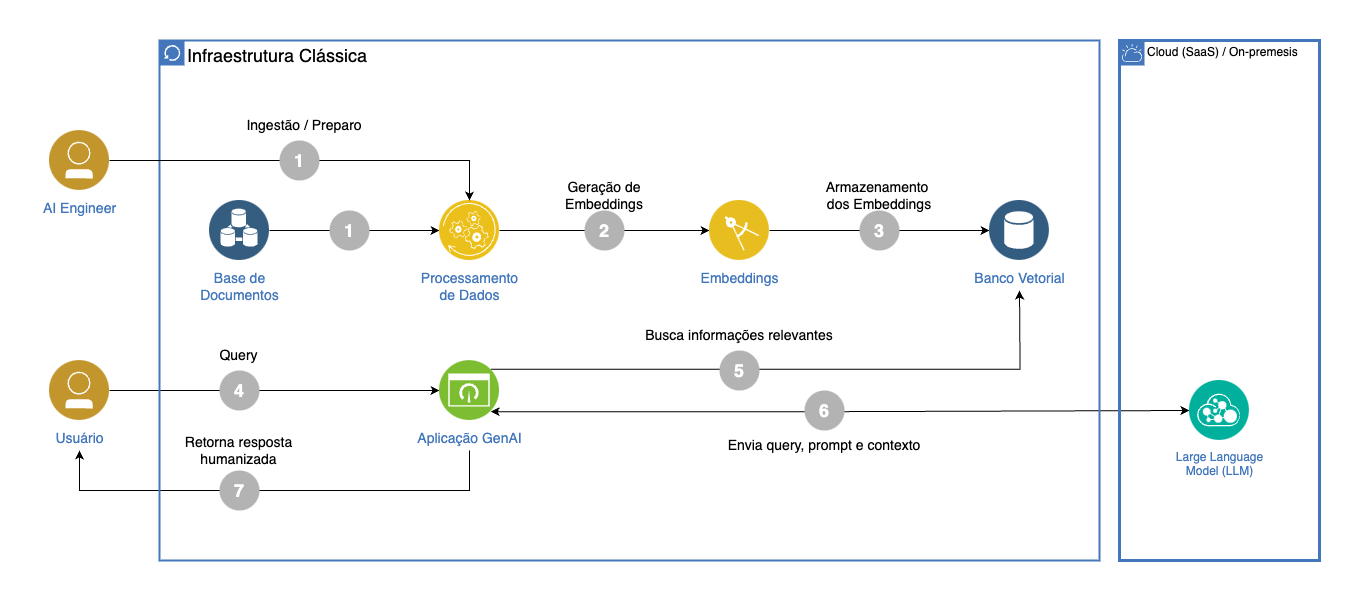
\includegraphics[scale=0.3]{architecture.png}
        \centering
        \caption{Visão arquitetural da solução RAG proposta para o trabalho}
        \centering
    \end{figure}

    \subsubsection{Ingestão e Preparo}
    
    Etapa onde a biblioteca é analisada, seus documentos são processados e transformados de maneira sequencial para obtermos um determinado modelo com as informações necessárias de cada documento. Esta etapa é dividida em duas partes, uma de ingestão e outra de preparo.

    \begin{itemize}
        \item Ingestão: Nesta parte os documentos são lidos e sua extensão é análisada, determinando a forma como o documento terá seus dados extraídos. Uma vez analisados, o documento é divididoo em chunks, um bloco de texto com os dados do documento.
        \item Preparo: Para cada chunk obtido na ingestão, é instanciado um modelo contendo os dados gerais do documento, assim como os dados do próprio chunk. Este modelo, em específico, visa uma inserção no banco vetorial que será feita na etapa de armazenamento dos embeddings.
    \end{itemize}

    \subsubsection{Geração de Embeddings}
    
    Antes de armazenar os modelos obtidos na etapa anterior, a informação de cada chunk precisa estar em um formato específico para o banco vetorial, este formato é obtido quando geramos os embeddings, que neste contexto, são uma representação numérica de baixa dimensão dos dados de um chunk expecífico.

    \subsubsection{Armazenamento dos Embeddings}
    
    Uma vez gerados, os embeddings de cada chunk estão presentes no modelo previamente adquirido na etapa de Ingestão e Preparo. Nesta etapa ocorre o armazenamento dos modelos na instância do banco vetorial do projeto. O armazenamento é feito de forma sequencial, porém em batches ou grupos com tamanho baseado na quantidade de chunks obtidos. Isso ocorre pois reduz o tempo da etapa de inserção ao banco, tendo em vista que uma vez que um documento é particionado em chunks, dependendo do tamanho do documento, podemos obter mais de 100 chunks, ou seja, 100 inserções.

    \subsubsection{Query}
    
    Aqui ocorre a interação do usuário com o sistema, nesta etapa o usuário digita uma pergunta dentro do espaço de input ou entrada da interface gráfica, que neste contexto é composta por um chat.

    \subsubsection{Busca por informações relevantes}
    
    No momento em que o usuário realiza a query, o sistema realiza uma busca por contexto ou informações relevantes como a biblioteca que o usuário está consultando (caso hajam múltiplas bibliotecas), uma determinada data, autor ou demais filtros que o usuário possa vir a fazer. Com as informações relevantes analisadas, é gerado um objeto de contexto que contém todas as informações relevantes

    \subsubsection{Envio de Query, Prompt e Contexto}
    
    Com o contexto e a query em mãos, o sistema prossegue com o fluxo principal e envia uma solicitação a API contendo a query que o usuário realizou, o prompt a ser seguido pela LLM e o contexto.

    \subsubsection{Retorno de Resposta Humanizada}
    
    Ao final da requisição feita pelo usuário, a API responde com uma lista contendo os objetos presentes no banco vetorial cujo embedding contém informações relevantes para a query do usuário. Esta lista contém os modelos presentes no banco vetorial, definidos na etapa de Preparação, e a partir dessa resposta passamos a lista para uma LLM que irá analisar primeiramente um prompt focado em entregar respostas humanizadas para o usuário. Neste prompt, há todo um cuidado para que qualquer desenvolvedor que deseje implementar este projeto possa utilizar do prompt engineering a fim de realizar as afinações necessárias para seu próprio contexto.

    \subsection{Tecnologias}

    \subsubsection{Python e Ambientes Virtuais}
    
    O Python 3.11 é uma das versões mais recentes da linguagem de programação Python, lançada com melhorias significativas em desempenho, novas funcionalidades e correções de bugs. Uma das principais inovações dessa versão é a otimização do tempo de execução, com um aumento significativo na velocidade em relação às versões anteriores, devido a melhorias no interpretador e na execução de código. Além disso, a versão 3.11 introduziu aprimoramentos na sintaxe, como a simplificação de anotações de tipos e novos recursos que facilitam o desenvolvimento de aplicativos mais robustos e eficientes. A linguagem continua a ser uma das mais populares, especialmente em áreas como desenvolvimento web, ciência de dados e inteligência artificial.
    
    Ambientes virtuais são espaços isolados onde é possível instalar e gerenciar dependências específicas de um projeto, sem afetar o sistema global ou outros projetos. Em Python, esses ambientes são criados com o módulo venv, permitindo que cada projeto tenha suas próprias versões de pacotes e bibliotecas. Isso evita conflitos entre dependências e facilita o gerenciamento de diferentes versões de pacotes para cada projeto.

    As principais vantagens dos ambientes virtuais incluem a capacidade de isolar dependências, garantindo que cada projeto utilize a versão correta de pacotes, a facilidade de replicar e compartilhar ambientes de desenvolvimento e a redução de problemas de compatibilidade entre pacotes ou versões do Python. Eles oferecem um controle mais preciso sobre o ambiente de execução, tornando o desenvolvimento mais seguro e eficiente.

    \subsubsection{Docling}
    Uma biblioteca Python projetada para facilitar a extração e organização de documentos. Ela permite que desenvolvedores processem automaticamente documentos de diferentes formatos, como PDFs, textos e arquivos de Word, para extrair informações estruturadas e relevantes. A biblioteca é útil para automatizar tarefas de leitura e processamento de grandes volumes de dados, organizando-os de forma a facilitar a análise posterior.

    A principal vantagem do Docling é a sua capacidade de simplificar o processo de extração de dados, tornando-o mais rápido e eficiente, sem a necessidade de escrever código complexo para lidar com diferentes tipos de documentos. Isso a torna uma ferramenta valiosa para projetos que requerem análise de texto ou a criação de bancos de dados a partir de documentos não estruturados.

    \subsubsection{Llama Index}
    Uma biblioteca Python que oferece ferramentas para criar índices eficientes, que podem ser usados em conjunto com modelos de linguagem, como o GPT, para realizar tarefas de busca e processamento de texto com alta performance.

    A principal vantagem do LlamaIndex é sua capacidade de organizar dados complexos de forma que seja fácil e rápido realizar consultas sobre eles, integrando-se bem com outras ferramentas de IA e processamento de linguagem natural. Isso a torna útil para criar soluções que necessitam de pesquisa e análise de grandes quantidades de informações, como em assistentes virtuais, sistemas de recomendação e análise de documentos.

    \subsubsection{Elastic Search}
    O ElasticSearch é um serviço de banco de dados baseado em busca de texto completo e análise de grandes volumes de dados. Ele é amplamente utilizado para armazenar, pesquisar e analisar dados de forma rápida e escalável. Baseado no motor de busca Apache Lucene, o ElasticSearch permite que dados sejam indexados e consultados com alta performance, suportando operações como pesquisa por palavras-chave, agregações e análises em tempo real.

    Em um banco vetorial, como o ElasticSearch, os dados são representados como vetores, o que permite consultas de similaridade, ou seja, encontrar documentos que sejam semanticamente semelhantes aos dados consultados. Isso é especialmente útil em casos de busca por texto, recomendação de conteúdo ou sistemas de recuperação de informações avançados. O ElasticSearch organiza e indexa esses vetores para proporcionar consultas eficientes e rápidas, sendo um componente essencial em sistemas que exigem grandes volumes de dados e análises complexas.

    \subsubsection{Ollama}
    A LLM do Ollama é uma ferramenta de inteligência artificial focada em fornecer modelos de linguagem avançados para tarefas como processamento de texto, geração de conteúdo, tradução, resumo e respostas a perguntas. Desenvolvido para ser altamente eficiente e acessível, o Ollama oferece modelos de linguagem que são otimizados para uma variedade de aplicações, desde automação de processos até assistência personalizada em diferentes domínios.

    A principal vantagem da LLM do Ollama é sua facilidade de integração em soluções de software, além de seu desempenho rápido e preciso. A plataforma é projetada para ser simples de usar, com uma interface intuitiva e suporte a diferentes linguagens de programação, tornando a tecnologia de IA mais acessível para desenvolvedores e empresas. Com um foco em flexibilidade e escalabilidade, o Ollama facilita a implementação de modelos de linguagem em larga escala sem comprometer a eficiência.

    \subsubsection{Fast API}
    Um framework moderno e de alto desempenho para construção de APIs em Python. Ele é baseado em padrões como Python type hints e pydantic, permitindo que desenvolvedores escrevam código de forma rápida e eficiente, com uma validação de dados robusta. O FastAPI se destaca pela sua velocidade, sendo capaz de processar requisições de maneira extremamente rápida, o que o torna ideal para aplicações que exigem alta performance.

    As principais vantagens do FastAPI incluem sua facilidade de uso, a validação automática de dados, a documentação interativa gerada com o Swagger UI, e sua performance comparável a frameworks como Node.js e Go. Além disso, o FastAPI aproveita os recursos de tipagem do Python, o que resulta em um código mais claro e com menos erros, além de ser altamente escalável e fácil de integrar com outras ferramentas.

    \subsubsection{Streamlit}
    Uma biblioteca em Python usada para criar interfaces web interativas de forma rápida e simples, sem a necessidade de conhecimentos avançados em desenvolvimento front-end. Ele permite que desenvolvedores criem dashboards, visualizações de dados e aplicativos interativos com poucos comandos, utilizando apenas Python. O Streamlit é ideal para protótipos rápidos e aplicativos que precisam integrar visualizações com análises de dados.

    As principais vantagens do Streamlit incluem sua simplicidade de uso, já que permite criar interfaces com poucas linhas de código, e sua integração direta com bibliotecas como Pandas, Matplotlib e Plotly, facilitando a visualização e análise de dados. Além disso, ele permite a criação de aplicativos interativos com atualizações em tempo real, sem a necessidade de configurar complexos sistemas de front-end. Isso torna o Streamlit uma opção excelente para cientistas de dados e desenvolvedores que desejam criar interfaces intuitivas sem precisar aprender HTML, CSS ou JavaScript.

    \clearpage

    \section{Solução Desenvolvida}
    \subsection{Visão Geral}
    \lipsum[1-2]
    \subsection{Funcionalidades}
    \lipsum[3-4]

    \clearpage

    \section{Conclusão}
    \subsection{Considerações Finais}
    \lipsum[1-2]
    \subsection{Limitações}
    \lipsum[3-4]
    \subsection{Trabalhos Futuros}
    \lipsum[5-6]

    \clearpage

    \section*{Referências}
    Instruções de bibliografia a seguir foram retiradas do manual de referência
    da Sociedade Brasileira de Computação \citeb{sbc}:
    % no meu TCC, eu utlizei somente \citep. Fale com seu supervisor.

    As referências bibliográficas devem ser de entendimento único e uniformes.
    Nós recomendamos dar ao autor nomes de referências em colchete, e.g.
    \citeb{knuth}, \citeb{smith};
    ou datas nos parênteses, \textcite{knuth}, \textcite{smith}.
    
    As referências devem ser listadas usando o tamanho de fonte de 12 pontos,
    com 6 pontos do espaço antes de cada referência.
    A primeira linha de cada referência não deve ser recuada,
    quando a subseqüente dever ser recuada 0.5 cm.
    \clearpage

    \nocite{*}

    % flush section font left
    \sectionfont{\raggedright}
    \printbibliography
    
\end{document}
